
\chapter{Getting Started}
\label{CH-GettingStarted}

Now that the config files are together we can get started. Open The vi WVDIAL\_Main.vi and start the main container. It should look like figure~\ref{Fig-StartupContainer}. All functionality of the container is within a tabular control. The first tab holds what you see now, and when an operation mode is selected the functionality associated with that mode will open up in tabs that were defined in the configure files associated with that mode. The main container also has some readout information near the bottom of the screen as well as three buttons for permissions, comments, and an abort. For relampago deployment the permissions and comments are not hooked up to anything, but the abort button is hooked up and will stop the labview program. When you want to stop labview operations make sure to stop the current running mode (usually main operations) wait for it to fully stop (all the tabs will go away and the buttons on the main tab will return) and then hit the abort button. Another feature that you will notice when entering an operational mode is a child responsivness display on the right hand side of the screen shown in figure~\ref{Fig-Responsive} and other options for running will become hidden as shown in figure~\ref{Fig-MainOpsContainer}. The child resonsivness display will show the children that are currently being used, and will confirm their responsivness to the main container. 

If any of these buttons doesn't seem to be working double check the config file corresponding to the operational mode attempting to be accessed. As a last effort a child can be called in stand alone mode. To do this first close the main container and then open the library that corresponds to the functionality desired, the child vi should be at the top of the list of the library. 

\begin{figure}[!ht]\centering
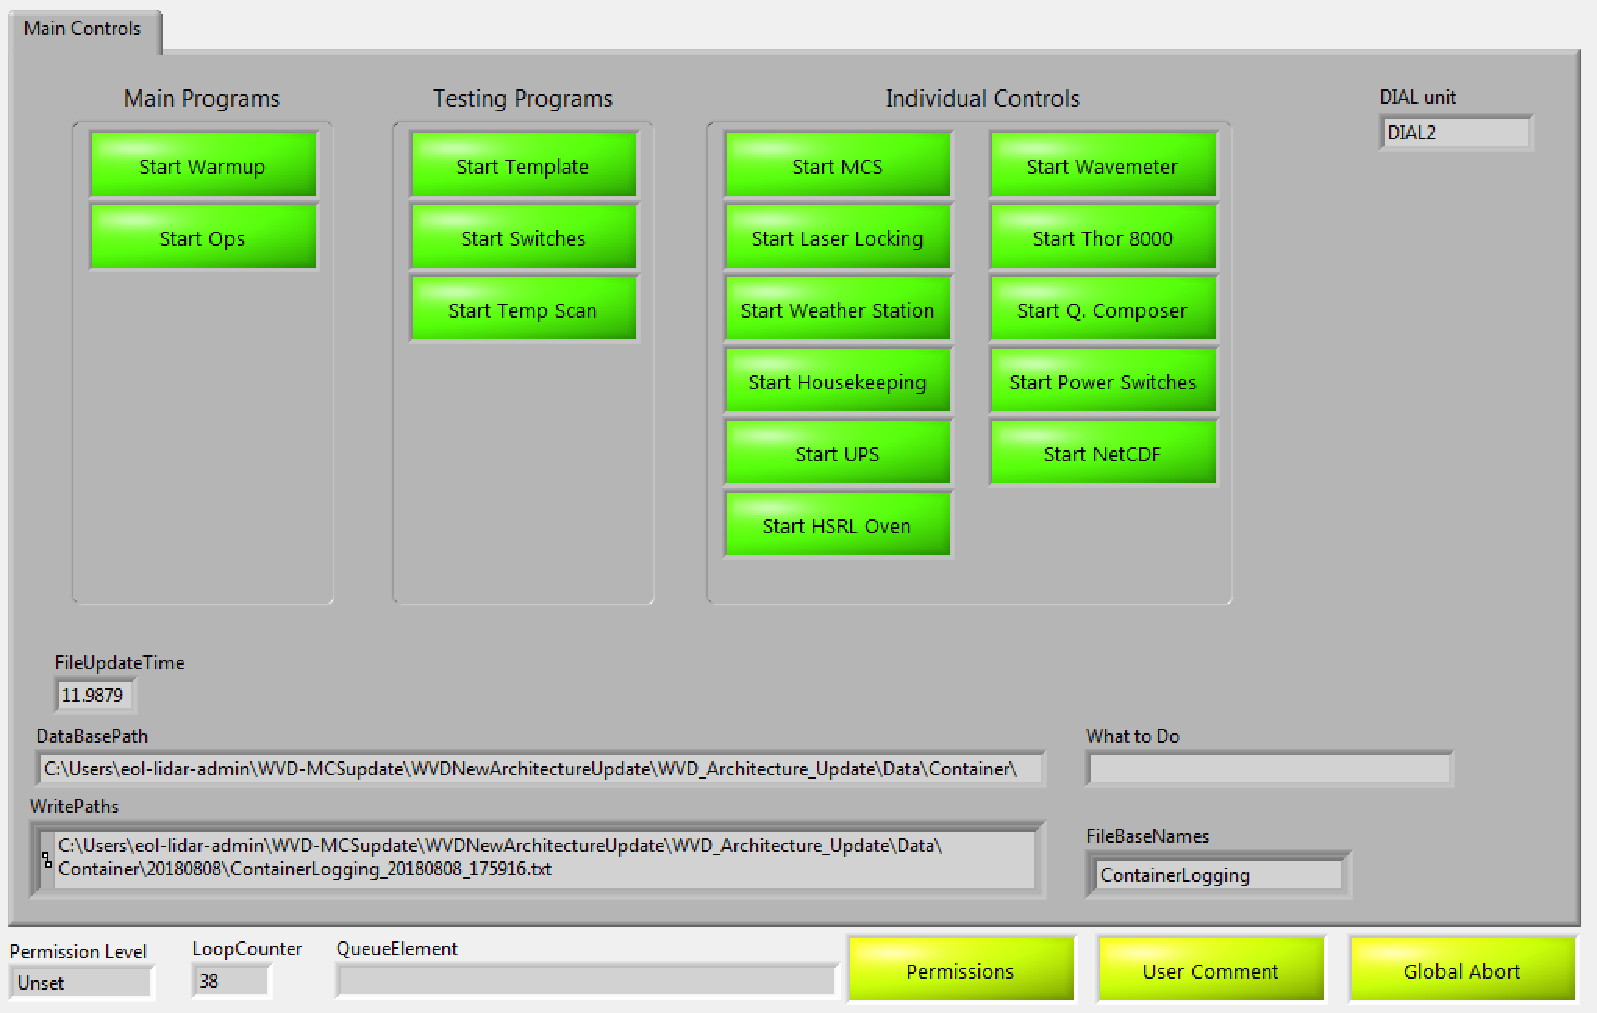
\includegraphics[height=3in]{Figures/StartupContainer}
\caption{The main container on startup.}
\label{Fig-StartupContainer}
\end{figure}


\begin{figure}[!ht]\centering
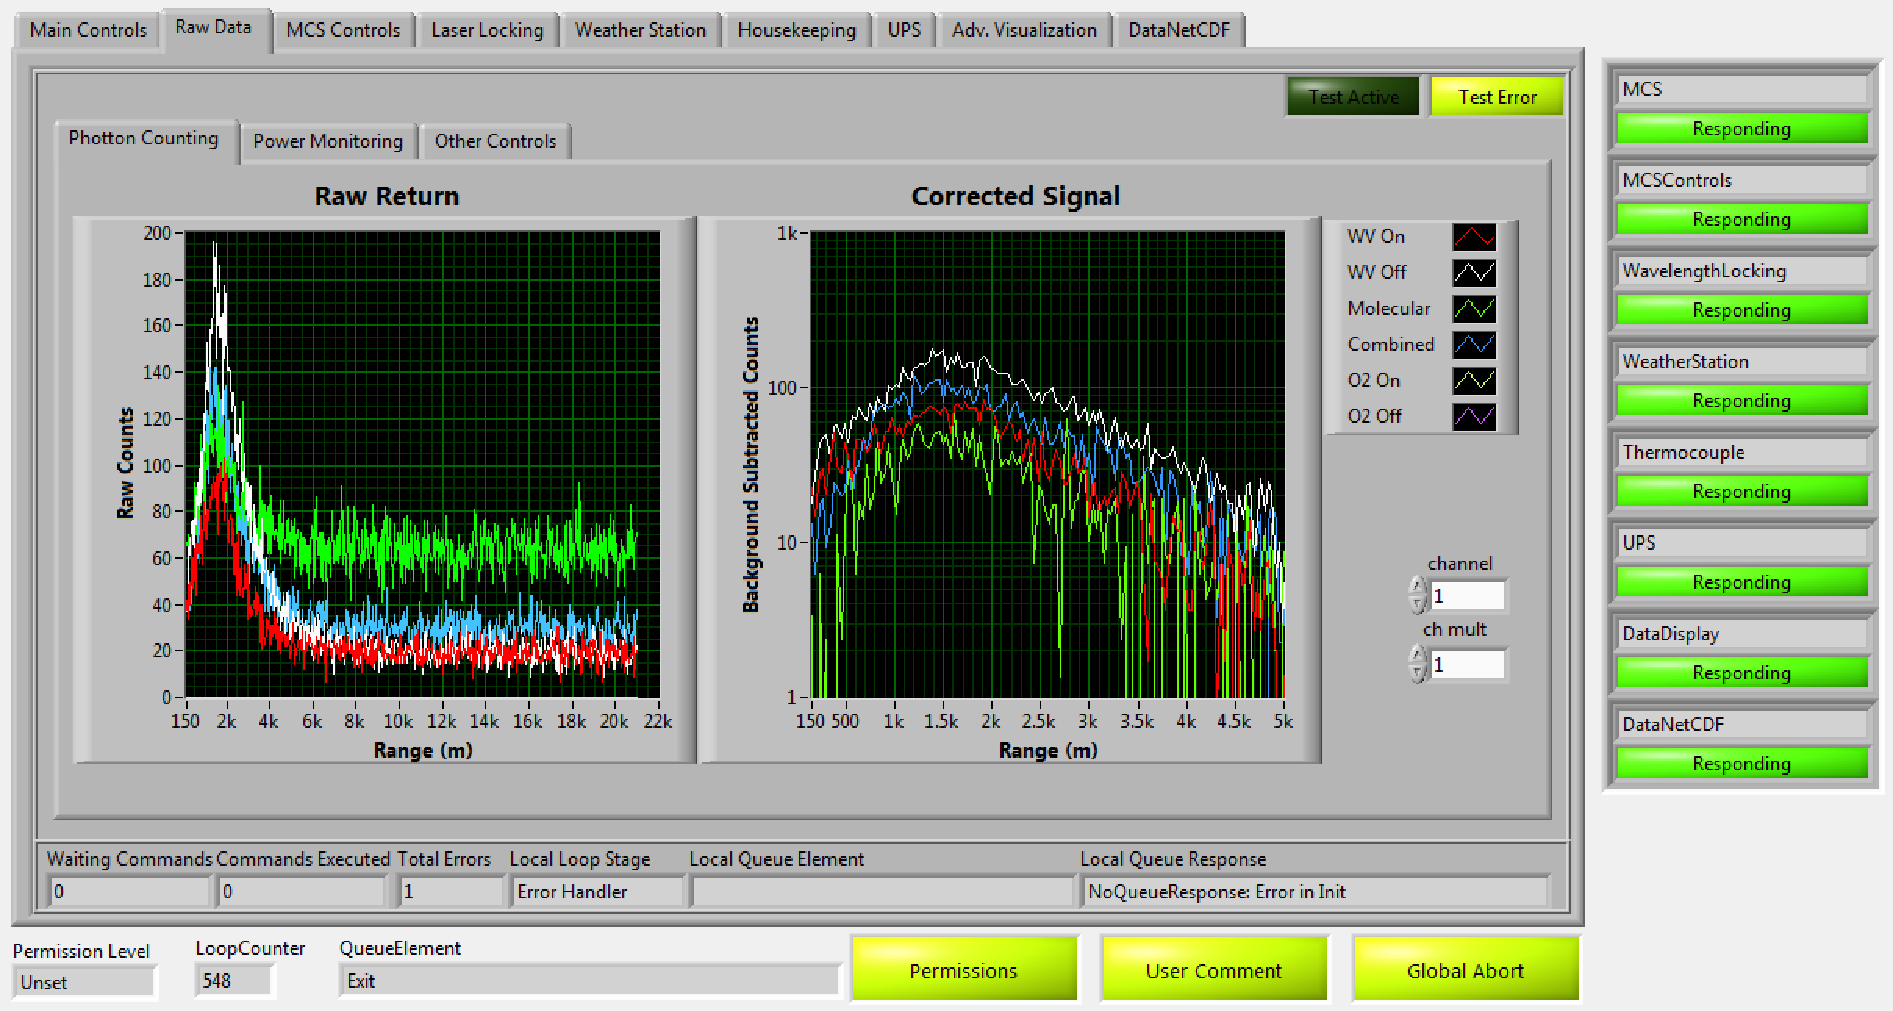
\includegraphics[height=3in]{Figures/MainOps}
\caption{The main container in MainOps mode.}
\label{Fig-MainOpsContainer}
\end{figure}

\begin{figure}[!ht]\centering
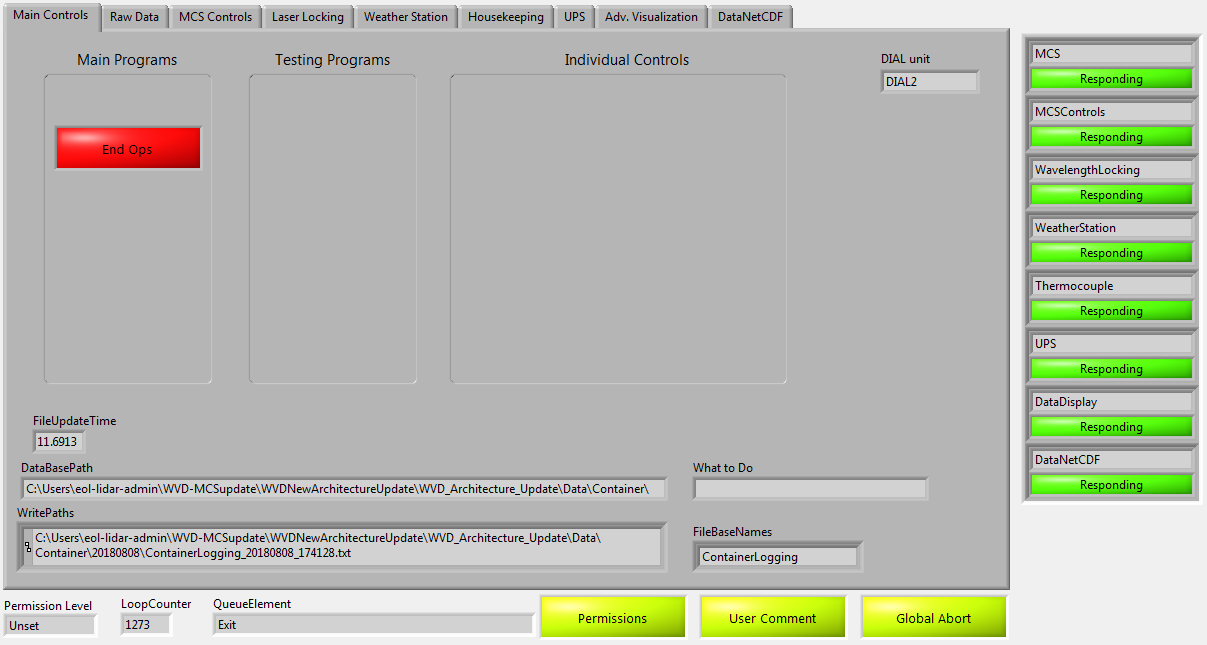
\includegraphics[height=3in]{Figures/MainOpsButtons}
\caption{The main container in ops mode with buttons hidden.}
\label{Fig-ContainerButtons}
\end{figure}

\begin{figure}[!ht]\centering
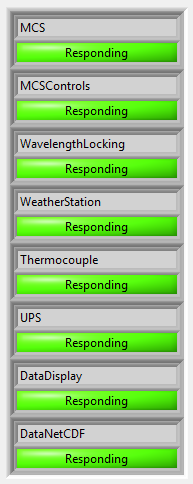
\includegraphics[height=3in]{Figures/RespondingReadout}
\caption{The display showing children as responsive.}
\label{Fig-Responsive}
\end{figure}

\newpage 
